\documentclass[10pt,UTF8]{ctexart}


\usepackage[margin=2cm,a4paper]{geometry}
%\usepackage[left=0.75in,top=0.6in,right=0.75in,bottom=1.0in,a4paper]{geometry}

\setmainfont{Caladea}
%% 也可以選用其它字庫:
% \setCJKmainfont[%
%   ItalicFont=AR PL KaitiM GB,
%   BoldFont=Noto Sans CJK SC,
% ]{Noto Serif CJK SC}
% setCJKsansfont{Noto Sans CJK SC}
% \renewcommand{\kaishu}{\CJKfontspec{AR PL KaitiM GB}}

% 繁體中文
\setCJKmainfont[Path=fonts/ ]{NotoSansTC-Medium.otf}

\usepackage{minted}
\usepackage[breaklinks]{hyperref}

% Picture
% 導言區的此三行無變化
\usepackage{graphicx}
\usepackage{float} 
\usepackage{subfigure}
% 以下是新增的自定義格式更改
\usepackage[]{caption2} %新增調用的宏包
\renewcommand{\figurename}{Fig.} %重定義編號前綴詞
\renewcommand{\captionlabeldelim}{.~} %重定義分隔符
 %\roman 是羅馬數字編號,\alph是默認的字母編號,\arabic是阿拉伯數字編號,可按需替換下一行的相應位置
\renewcommand{\thesubfigure}{(\roman{subfigure})}%此外,還可設置圖編號顯示格式,加括號或者不加括號
\makeatletter \renewcommand{\@thesubfigure}{\thesubfigure \space}%子圖編號與名稱的間隔設置
\renewcommand{\p@subfigure}{} \makeatother

% Math
\usepackage {mathtools}
\usepackage{amssymb}

% Code
\usepackage{listings}
\usepackage{xcolor}
\lstset{
    % backgroundcolor=\color{red!50!green!50!blue!50},
    % 程式碼塊背景色為淺灰色
    rulesepcolor= \color{gray}, % 程式碼塊邊框顏色
    breaklines=true,  % 程式碼過長則換行
    numbers=left, % 行號在左側顯示
    numberstyle= \small,% 行號字型
    % eywordstyle= \color{red,% 關鍵字顏色
    commentstyle=\color{gray}, % 註釋顏色
    frame=shadowbox % 用方框框住程式碼塊
    }

\usepackage{hyperref}

\title{算法分析和複雜性理論}
\author{干皓丞,2101212850, 信息工程學院}

\begin{document}
\maketitle


\section{作業目標與章節摘要}

1. LeetCode 240. Search a 2D Matrix II 搜索二維矩陣 II

2. LeetCode 347. Top K Frequent Elements 前 K 個高頻元素

3. LeetCode 374. Guess Number Higher or Lower 二叉樹的所有路徑


\section{作業內容概述}

作業可以從 GitHub 下的 kancheng/kan-cs-report-in-2022 專案找到,作業程式碼與文件目錄為 kan-cs-report-in-2022/AATCC/lab-report/。實際執行的環境與實驗設備為 Google 的 Colab 、MacBook Pro (Retina, 15-inch, Mid 2014) 、 Acer Aspire R7 與 HP Victus (Nvidia GeForce RTX 3060)。

本作業 GitHub 專案為 kancheng/kan-cs-report-in-2022 下的 AATCC` 的目錄。程式碼可以從 code 目錄下可以找到 *.pynb,內容包含上次課堂練習、LeetCode 範例思路整理與作業。

https://github.com/kancheng/kan-cs-report-in-2022/tree/main/AATCC

\begin{figure}[H]
\centering 

\includegraphics[width=0.30\textwidth]{aatccqr.png} 
\caption{作業專案位置}
\label{Test}
\end{figure}


1. LeetCode : https://leetcode.com/

2. LeetCode CN : https://leetcode-cn.com/

3. OnlineGDB : https://www.onlinegdb.com/ 

LeetCode 的平台部分, CN 的平台有針對簡體中文使用者進行處理,包含中英文切換等功能。OnlineGDB 則可線上進行簡易的環境測試,其程式碼涵蓋 C, C++, C\#, Java, Python, JS, Rust, Go。

\newpage

\section{LeetCode 240. Search a 2D Matrix II 搜索二维矩阵 II}

\subsection{LeetCode 240. 題目}


Write an efficient algorithm that searches for a value target in an m x n integer matrix matrix. This matrix has the following properties:

- Integers in each row are sorted in ascending from left to right.

- Integers in each column are sorted in ascending from top to bottom.

編寫一個高效的算法來搜索 m x n 矩陣 matrix 中的一個目標值 target 。該矩陣具有以下特性:

- 每行的元素從左到右升序排列。

- 每列的元素從上到下升序排列。

\begin{figure}[H]
\centering 
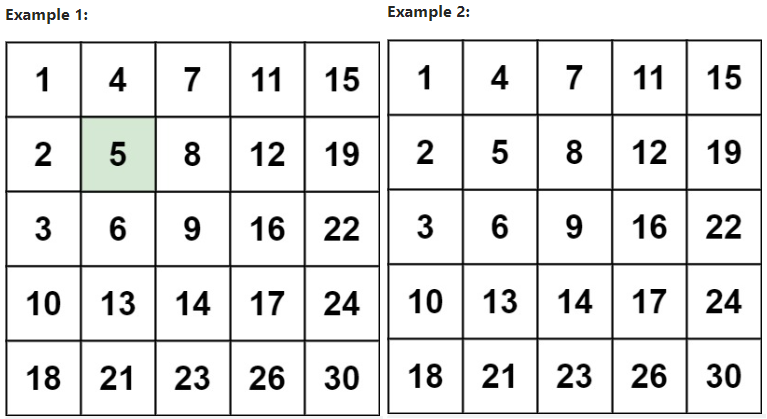
\includegraphics[width=0.80\textwidth]{lc-240-p-example.png} 
\caption{Example}
\label{Test}
\end{figure}

Example 1:

\begin{lstlisting}[language={python}]
Input: matrix = [[1,4,7,11,15],[2,5,8,12,19],[3,6,9,16,22],[10,13,14,17,24],[18,21,23,26,30]], target = 5
Output: true
\end{lstlisting}


Example 2:

\begin{lstlisting}[language={python}]
Input: matrix = [[1,4,7,11,15],[2,5,8,12,19],[3,6,9,16,22],[10,13,14,17,24],[18,21,23,26,30]], target = 20
Output: false
\end{lstlisting}


Constraints:

1. m == matrix.length

2. n == matrix[i].length

3. 1 <= n, m <= 300

4. $-10^{9} <= matrix[i][j] <= 10^{9}$

5. All the integers in each row are sorted in ascending order.

6. All the integers in each column are sorted in ascending order.

7. $-10^{9} <= target <= 10^{9}$


\subsection{LeetCode 240. 思路總結}

1. 給出一個二維矩陣,矩陣的特點是每一個行內,元素隨著下標增大而增大,每一列內,元素也是隨著下標增大而增大。但是相鄰兩行的元素並沒有大小關係。例如第一行最後一個元素就比第二行第一個元素要大。要求設計一個算法能在這個矩陣中高效的找到一個數,如果找到就輸出 true,找不到就輸出 false。

2. 這一題是第 74 題的加強版。第 74 題中的二維矩陣完全是一個有序的一維矩陣,但是這一題如果把它拍扁成一維,並不是有序的。首先每一個行或者每一列是有序的 ,那麼我們可以依次在每一行或者每一列中利用二分去搜索。這樣做時間複雜度為 O(n log n)。

3. 還有一個模擬的解法。通過觀察,我們發現了這個矩陣的一個特點,最右邊一列的元素是本行中最大的元素,所以我們可以先從最右邊一列開始找到第一個比 target 元素大的元素,這個元素所在的行,是我們接著要搜索的。在行中搜索是從最右邊開始往左邊搜索,時間複雜度是 O(n),算上一開始在最右邊一列中查找的時間複雜度是 O(m),所以最終的時間複雜度為 O(m+n)。

\subsection{LeetCode 240. Code 範例}

\begin{lstlisting}[language={python}]
class Solution:
    def searchMatrix(self, matrix, target):
        """
        :type matrix: List[List[int]]
        :type target: int
        :rtype: bool
        """
        m = len(matrix)
        if m == 0:
            return False
        n = len(matrix[0])
        if n == 0:
            return False

        i = m - 1
        j = 0
        while i >= 0 and j < n:
            if matrix[i][j] == target:
                return True
            elif matrix[i][j] < target:
                j = j + 1
            else:
                i = i - 1
        return False
\end{lstlisting}

\subsection{LeetCode 240. 結果}

\begin{figure}[H]
\centering 
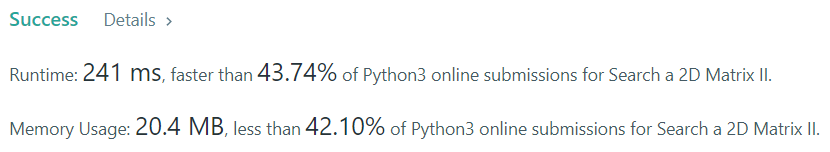
\includegraphics[width=0.80\textwidth]{lc-240-o.png} 
\caption{LeetCode 240 結果}
\label{Test}
\end{figure}


\newpage

\section{LeetCode 347. Top K Frequent Elements 前 K 个高频元素}

\subsection{LeetCode 347. 題目}

Given an integer array nums and an integer k, return the k most frequent elements. You may return the answer in any order.

給你一個整數數組 nums 和一個整數 k ,請你返回其中出現頻率前 k 高的元素。你可以按 任意順序 返回答案。

Example 1:

\begin{lstlisting}[language={python}]
Input: nums = [1,1,1,2,2,3], k = 2
Output: [1,2]
\end{lstlisting}

Example 2:

\begin{lstlisting}[language={python}]
Input: nums = [1], k = 1
Output: [1]
\end{lstlisting}

Constraints:

- $1 <= nums.length <= 10^{5}$

- k is in the range [1, the number of unique elements in the array].

- It is guaranteed that the answer is unique.


\subsection{LeetCode 347. 思路總結}

把數組構造成一個優先隊列,輸出前 K 個即可。

\subsection{LeetCode 347. Code 範例}

\begin{lstlisting}[language={python}]
from typing import List 
import heapq
class Solution:
    def topKFrequent(self, nums: List[int], k: int) -> List[int]:
        map_ = {}
        for i in range(len(nums)):
            map_[nums[i]] = map_.get(nums[i], 0) + 1
        pri_que = []
        for key, freq in map_.items():
            heapq.heappush(pri_que, (freq, key))
            if len(pri_que) > k: 
                heapq.heappop(pri_que)
        result = [0] * k
        for i in range(k-1, -1, -1):
            result[i] = heapq.heappop(pri_que)[1]
        return result 
\end{lstlisting}

\subsection{LeetCode 347. 結果}

\begin{figure}[H]
\centering 
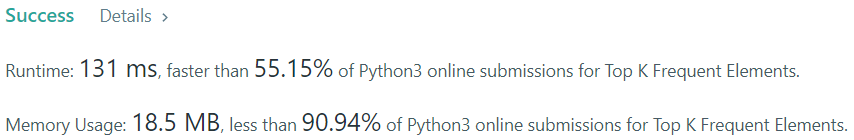
\includegraphics[width=0.80\textwidth]{lc-347-o.png} 
\caption{LeetCode 347 結果}
\label{Test}
\end{figure}


\newpage

\section{LeetCode 374. Guess Number Higher or Lower 二叉树的所有路径}

\subsection{LeetCode 374. 題目}

We are playing the Guess Game. The game is as follows:

I pick a number from 1 to n. You have to guess which number I picked.

Every time you guess wrong, I will tell you whether the number I picked is higher or lower than your guess.

You call a pre-defined API int guess(int num), which returns three possible results:

- -1: Your guess is higher than the number I picked (i.e. num > pick).

- 1: Your guess is lower than the number I picked (i.e. num < pick).

- 0: your guess is equal to the number I picked (i.e. num == pick).

Return the number that I picked.

猜數字遊戲的規則如下:

每輪遊戲,我都會從 1 到 n 隨機選擇一個數字。請你猜選出的是哪個數字。
如果你猜錯了,我會告訴你,你猜測的數字比我選出的數字是大了還是小了。
你可以通過調用一個預先定義好的接口 int guess(int num) 來獲取猜測結果,返回值一共有 3 種可能的情況(-1,1 或 0):

-1:我選出的數字比你猜的數字小 pick < num
1:我選出的數字比你猜的數字大 pick > num
0:我選出的數字和你猜的數字一樣。恭喜!你猜對了! pick == num

返回我選出的數字。

Example 1:

\begin{lstlisting}[language={python}]
Input: n = 10, pick = 6
Output: 6
\end{lstlisting}

Example 2:

\begin{lstlisting}[language={python}]
Input: n = 1, pick = 1
Output: 1
\end{lstlisting}

Example 3:

\begin{lstlisting}[language={python}]
Input: n = 2, pick = 1
Output: 1
\end{lstlisting}

Constraints:

- 1 <= n <= $2^31$ - 1

- 1 <= pick <= n



\subsection{LeetCode 374. 思路總結}

二分查找

\subsection{LeetCode 374. Code 範例}

\begin{lstlisting}[language={python}]
class Solution:
    def guessNumber(self, n: int) -> int:
        left ,right = 1,n
        while left <= right:
            mid = (left + right) // 2
            if guess(mid) == 1:
                left = mid + 1
            elif guess(mid) == -1:
                right = mid - 1
            else :
                return mid
\end{lstlisting}

\subsection{LeetCode 374. 結果}

\begin{figure}[H]
\centering 
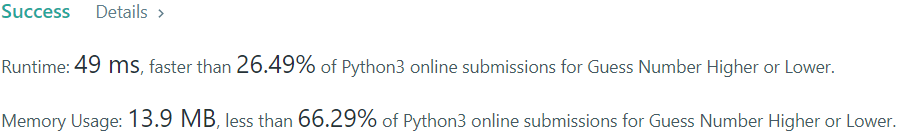
\includegraphics[width=0.80\textwidth]{lc-374-o.png} 
\caption{LeetCode 374 結果}
\label{Test}
\end{figure}



%\section{附錄}

% 數學意義說明

% $$\min \limits_{G}\max \limits_{D}{V_I(D,\ G)=V(D,G)-\lambda L_I(G,Q)}$$

%	\begin{lstlisting}[language={python}]

%	\end{lstlisting}

%\begin{enumerate}
%\item Y
%\item A
%\end{enumerate}

% \newpage

\clearpage

\end{document}